\documentclass[10pt,twocolumn,letterpaper]{article}

\usepackage{cvpr}
\usepackage{times}
\usepackage{epsfig}
\usepackage{graphicx}
\usepackage[font=small,labelfont=bf]{caption}
\usepackage{wrapfig}
\usepackage{booktabs}
\usepackage{subfig}
\usepackage{amsmath}
\usepackage{amssymb}
%
\newcommand{\tnote}[3]{{\color{#2}#1: #3}}
\newcommand{\change}[1]{\textcolor{red}{#1}}
\newcommand{\DaH}[1]{\tnote{DaH}{red}{#1}}
\newcommand{\VKF}[1]{\tnote{VKF}{green}{#1}}
\newcommand{\JT}[1]{\tnote{JT}{blue}{#1}}
\newcommand{\IGNORE}[1]{}
% Include other packages here, before hyperref.

% If you comment hyperref and then uncomment it, you should delete
% egpaper.aux before re-running latex.  (Or just hit 'q' on the first latex
% run, let it finish, and you should be clear).
\usepackage[pagebackref=true,breaklinks=true,letterpaper=true,colorlinks,bookmarks=false]{hyperref}

% \cvprfinalcopy % *** Uncomment this line for the final submission

\def\cvprPaperID{****} % *** Enter the CVPR Paper ID here
\def\httilde{\mbox{\tt\raisebox{-.5ex}{\symbol{126}}}}

% Pages are numbered in submission mode, and unnumbered in camera-ready
\ifcvprfinal\pagestyle{empty}\fi
\begin{document}

%%%%%%%%% TITLE
\title{Guided Proofreading of Automatic Segmentations in Connectomics}

\author{First Author\\
Institution1\\
Institution1 address\\
{\tt\small firstauthor@i1.org}
% For a paper whose authors are all at the same institution,
% omit the following lines up until the closing ``}''.
% Additional authors and addresses can be added with ``\and'',
% just like the second author.
% To save space, use either the email address or home page, not both
\and
Second Author\\
Institution2\\
First line of institution2 address\\
{\tt\small secondauthor@i2.org}
}

\maketitle
%\thispagestyle{empty}

%%%%%%%%% ABSTRACT
\begin{abstract}
Automatic cell image segmentation methods in connectomics can lead to \emph{split} and \emph{merge} errors, which require correction through proofreading. To aid error correction, we develop two classifiers that are able to recommend candidate errors and their corrections to the user. These classifiers are informed by training a convolutional neural network with known errors in automatic segmentations by comparison to expert-labeled ground truth. Our network architecture is able to detect potentially erroneous regions by considering a large context region around a segmentation boundary. With recommendations, proofreading of mouse cortex electron microscopy image segmentations can reduce VI scores from 0.476 to 0.426, which we find is an improvement on pure manual and pure automatic cases that both cause VI to increase.
\end{abstract}

\input{1.introduction} % Now contains related work
%\section{Related Work}

\paragraph{Automatic Segmentation}

Multi-terabyte EM brain volumes require automatic segmentation~\cite{jain2010,Liu2014,NunezIglesias2013Machine,GALA2014}, but can be hard to classify \change{due to ambiguous intercellular space: the 2013 IEEE ISBI neurites 3D segmentation challenge~\cite{isbi_challenge} showed that existing algorithms which learn from expert-segmented training data still exhibit high error rates.}

NeuroProof \cite{neuroproof2013} \change{tries to decrease error rates} with interactive learning of agglomeration of over-segmentations of images, based on a random forest classifier. Vazquez-Reina et al.~\cite{amelio_segmentation} propose automatic 3D segmentation by taking whole EM volumes into account rather than a per section approach, then solving a fusion problem with a global context. Kaynig et al.~\cite{kaynig10} propose a random forest classifier coupled with an anisotropic smoothing prior in a conditional random field framework with 3D segment fusion. It is also possible to learn segmentation classification features directly from images with CNNs. Ronneberger et al.~\cite{RonnebergerFB15} use a contracting/expanding CNN path architecture to enable precise boundary localization with small amounts of training data. Lee et al.~\cite{lee2015recursive} recursively train very deep networks with 2D and 3D filters to detect boundaries. 

\change{These approaches make good progress; however, in general, proofreading is required to improve them through generating more ground-truth segmentations.}

% JT: Feels out of place...
Arganda-Carreras et al.~\cite{10.3389/fnana.2015.00142} posed the ISBI 2D EM segmentation challenge in 2012, where a 30-image corpus of fly cell `in/out' labels was used to train boundary detection. However, mouse brain EM data is more difficult than the ISBI 2012 challenge, as it contains significant intercellular space which is hard to classify.

Bogovic et al.~\cite{BogovicHJ13} learn 3D features, and show even that unsupervised learning can produce better features than hand-designs. We extend the features reported by Bogovic et al.\ but limit the classification to 2D images rather than 3D. In this case, reconstruction is unnecessary and, instead of waiting for the alignment of the 3D output, proofreading can start immediately to maximize throughput.

\paragraph{Collaborative Interactive Segmentation}

Recent works attack the problem of massive volume segmentation through crowd-sourcing\cite{saalfeld09,anderson2011}. EyeWire~\cite{eyewire2012} asks novice users to participate in a segmentation game with neuronal structures using a semi-automatic algorithm. D2P ~\cite{Giuly2013DP2} uses a micro-labor workforce approach where local boolean decisions are combined to produce a consensus segmentation. In general, our goal is to correct the output of a segmentation which is thought to be good; hence, our tool would be used after learning a segmentation model to direct user attention to correct likely erroneous areas.

\paragraph{Proofreading Tools}
\change{The editing bottleneck for existing imperfect automatic segmentations} was identified by Peng et al. \cite{proofreading_bottleneck}. The authors developed software which supports three-dimensional proofreading. Also for 3D, Sicat et al. proposed a graph abstraction method to guide users to problematic regions indicating the need for corrections \cite{markus_proofreading}. Janelia Farms then introduced Raveler \cite{raveler}, a software targeting expert users by offering many parameters for tweaking the proofreading process at the cost of a higher complexity. Raveler also includes a simple 3D renderer to validate corrections across slices.

\change{In 2014, Haehn et al.\ developed two proofreading tools: Mojo and Dojo. Mojo provides a simple scribble interface for error correction, and Dojo extends this for distributed proofreading via a minimalistic web-based user interface. The authors defined requirements for general proofreading tools, and then evaluated the accuracy and speed of Raveler, Mojo, and Dojo through a quantitative user study (Sec. 3 and 4) \cite{haehn_dojo_2014}.}
Al-Awami et al.\ integrated Dojo into the Neuroblocks proofreading management system \cite{Neuroblocks}, which tracks and visualizes progress among multiple users.

In 2015, Karimov et al.\ proposed a guided volume editing approach using histogram dissimilarity \cite{karimov_guided_volume_editing}. Measuring differences in histogram distributions helps to find potential errors and to suggest possible corrections. These promising results on Computed-Tomography Angiography datasets are targeted towards expert users.

Recently, Uzunbas et al.\ showed that potential labeling errors can be found by considering the merge tree of an automatic segmentation method \cite{uzunbas}. The authors track uncertainty through automatic labeling and then present potential regions for proofreading. This requires access to the segmentation merge tree, which is not always available.


%\subsection{Contributions}

%Given this, we contribute to the literature:
%\begin{enumerate}
%\item One contribution
%\item Two contribution
%\item (Maybe) three contribution
%\end{enumerate}
\begin{figure}[t]
 \centering
    \subfloat[CNN Layers\label{fig:layers}]{%
      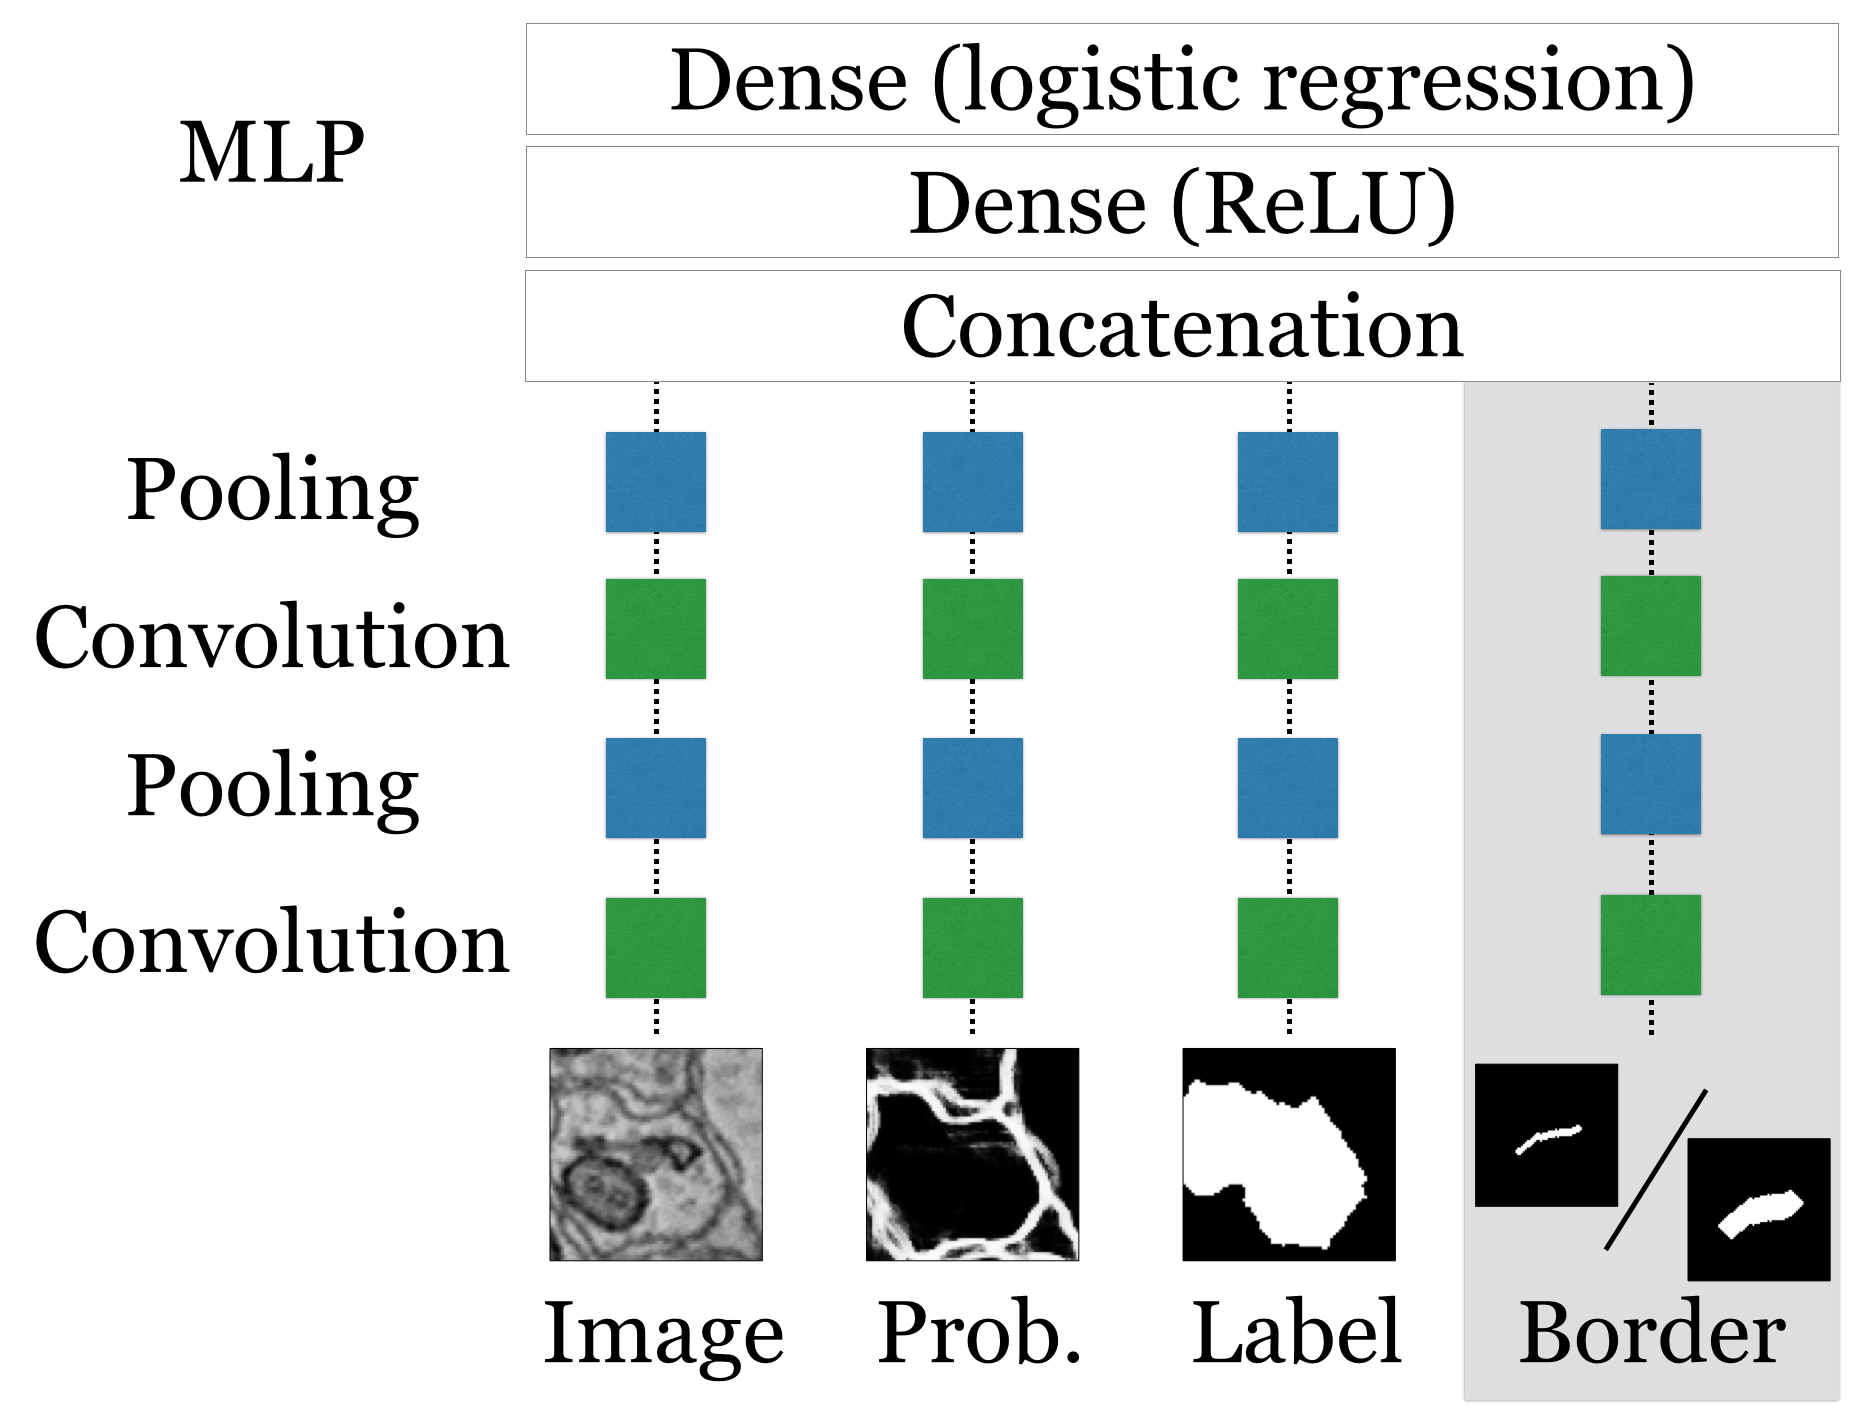
\includegraphics[width=0.9\textwidth]{gfx/network.png}
    }

    \subfloat[Network configurations\label{fig:networks}]{%
      \includegraphics[width=0.9\textwidth]{gfx/network_inputs.png}
    }
	\caption{(a) Our network architecture with up to four input channels, each with two convolutional and two pooling layers. MergeNet includes four separate input channels and RGBANet uses a 4-channel input. (b) We trained three different network configurations with three and four inputs: A) image, boundary map probability, and merged binary mask; B) A configuration extended with a small border mask, to focus on the specific boundary in question; C) A configuration extended with a large border mask.}

\end{figure}

\section{Method}
%Paragraph one: Overview of the method. What are the high level steps taken to build the system? What are the key techniques used within the system?
We build a split error classifier using a convolutional neural network (CNN) to check the boundaries of an existing automatic segmentation. For each boundary, the CNN provides a probability that points sampled along the boundary caused a split error. For each boundary, we sample up to 10 decision points, where the decision points are spread evenly over the boundary length, so long as their context windows do not overlap. These probabilities are then weighted by the length of the boundary within the context over the total boundary length, and averaged. A greedy algorithm then merges neighboring regions sequentially, starting with the highest probability score. Following each merge, neighboring boundaries are re-evaluated for split errors. Correcting a split error is as simple as merging the two bordering labels.

Identification and correction of merge errors is more challenging, because we must look inside segmentation regions for missing or incomplete boundaries and then propose the correct boundary. However, we can reuse the same trained CNN for this task. For each segmentation label, we generate 30 potential boundaries through the region by placing watershed seed points at opposite sides of the label boundary and generating the corresponding split. Then, we check to see whether any potential edge is classified as a split error. If the CNN detects a boundary with a very low split error score, then the boundary should have been in the segmentation and the region is a candidate for a merge error.
%\JT{Candidate for figure - this potential boundary generation is a bit tricky to follow.}\VKF{Maybe put some more candidates into Figure 1 as examples?}



%\begin{figure}[t]
%\centering
%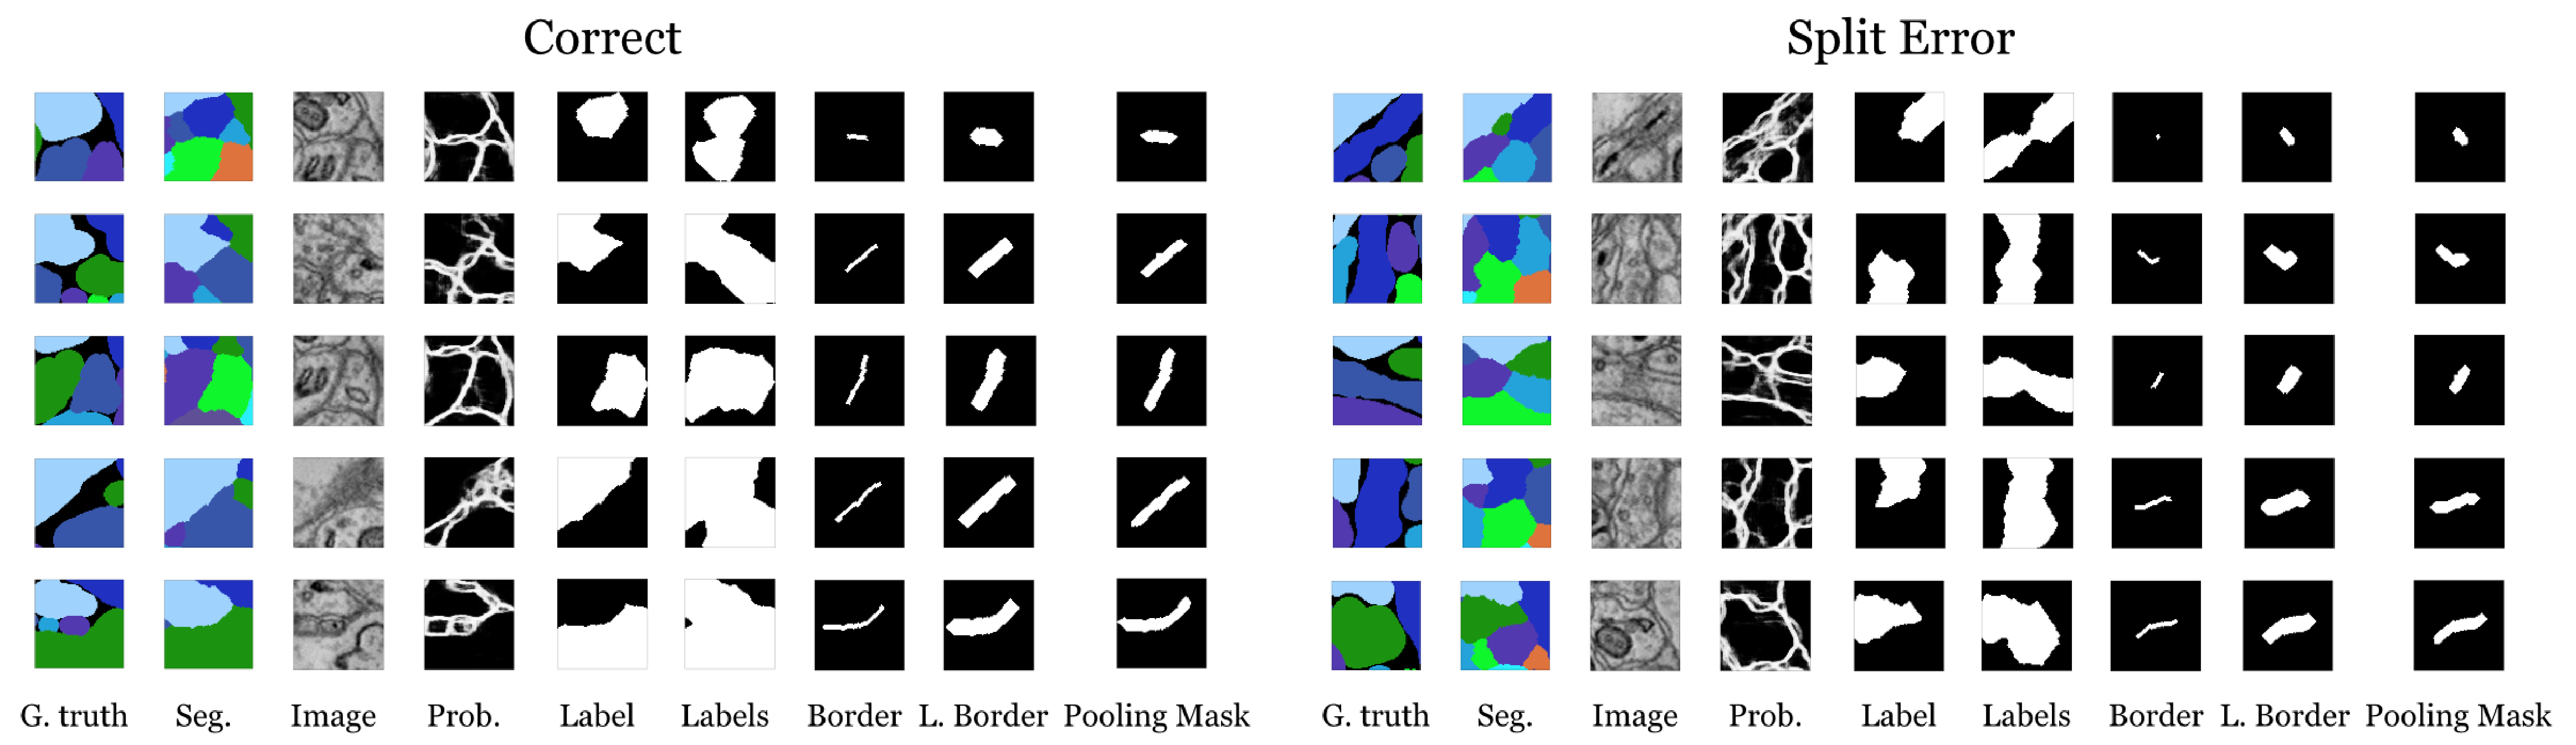
\includegraphics[scale=.15]{gfx/patches.pdf}
%\caption{\JT{NEW CAPTION PLEASE.}}
%\label{fig:patches}
%\end{figure}




\subsection{Convolutional Neural Network Design}
%Paragraph: What is the rationale behind our network design? Why do we think this will work over other approaches?
To train a CNN for split error detection we take multiple channels of context information of the boundary into consideration for the decision making process. We pass multiple inputs into the CNN windowed around a particular decision point or pixel: the input grayscale image patch, the corresponding boundary probability map patch, and two corresponding binary mask patches for the segmented regions at either side of the boundary. Following Bogovic et al.~\cite{BogovicHJ13}, these two masks can be combined into a single mask with comparable performance (configuration A, Fig.~\ref{fig:networks}). The network then leverages these multiple input patches to identify and correct errors made by the previous membrane detection network and automatic segmentation pipeline.

One way to combine these inputs is to treat them as a 4-channel input, so that alignment between the input image and the segmentation masks are not lost throughout the convolutions. We refer to this approach as \textit{RGBANet}. However, training a boundary-classifying network can be difficult due to rigid ground-truth segmentations, which often differ substantially from automatic segmentation regions in ambiguous extra-cellular space. To cope with this variation, our network is based on multiple separate input channels (Fig.~\ref{fig:layers}). Each of the input patches is connected individually to a 2-layer network, with each layer consisting of convolutional and pooling layers. The output of these networks is then combined by a fully connected multi-layer perceptron (MLP) with one hidden layer and a two class logistic regression output layer. The intuition for this multiple input channel approach is that we want to allow variation in the input and masks independently, to accommodate potential error, and then for the hidden layers to discover appropriate combinations of the relevant features learned separately for the different input channels. We refer to this approach as \textit{MergeNet}.

To better direct both networks to train on the true boundary edge, which in many cases is missing from the boundary probability map and hence is the cause of merge errors, we additionally pass as input a second binary mask. This mask contains the true boundary edge (configuration B, Fig.~\ref{fig:networks}). To consider slight edge ambiguities, we also test a version of this network where the true boundary mask has been dilated by 5 pixels (configuration C).

% \VKF{DELETE RIGHT? Another change is in the pooling layer itself. Bogovic et al.~\cite{BogovicHJ13} designed an unsupervised learning approach for agglomerative clustering of oversegmentations, using dynamic pooling of features extracted around objects and boundaries to increase performance. Inspired by their call for a supervised learning equivalent, we integrate a pooling layer into our CNN which is similar in spirit to their unsupervised approach. Instead of conventional max- or avg-pooling where a sliding window is equally applied to the whole output of the convolutional layer, our dynamic pooling only averages outputs within a region of interest. We implemented both pooling methods and compared them ???} 


%  
%    \begin{subfig}[b]{0.5\textwidth}
%        \includegraphics[scale=.15]
%        \caption{CNN Layers}
%        \label{fig:layers}
%    \end{subfigure}
%    \begin{subfigure}[b]{0.5\textwidth}
%        \includegraphics[scale=.15]
%        \caption{Different Network Configurations}
%        \label{fig:networks}
%    \end{subfigure}    
%\missingfigure{Network architecture figure}


\subsection{Training}
To train the network, we use the blue 3-cylinder mouse cortex volume of Kasthuri et al. \cite{kasthuri2015saturated} (2048 x 2048 x 300 voxels). The tissue is dense mammalian neuropil from layers 4 and 5 of the S1 primary somatosensory cortex of a healthy mouse. The resolution of our data set is $3\, nm$ per pixel, and the section thickness is $30\, nm$. 
%\VKF{For the initial automatic segmentation, we train an existing pipeline on a similar data set}. 
A manually-labeled expert segmentation is available as a ground truth for the entire data set. We use the first 250 sections of the data for training and validation (split 0.25) and the last 50 for testing. To generate training data, we identify correct regions and split errors in the automatic segmentation by intersecting with the ground truth regions. From these regions, we sample 266,088 correct regions and 266,088 split error patches. As patch size, we defined $75 x 75$ pixels to cover $\approx80\%$ of all boundaries in our segmentation output. 
%#   Training data:
%#   Patch size: (75,75)
%#   79828 correct splits
%#   79828 split errors
%#   rotated 90,180,270 degrees after each epoch
%
%#   validation data: 7464 correct splits + 7464 split errors
%#   test data: 5748 correct splits + 5748 split errors


\begin{figure*}
%\ffigbox[][\textwidth]{
%\begin{floatrow}

\includegraphics[width=.5\textwidth]{gfx/roc_plot.pdf}


\begin{tabular}{l rrrr}
\toprule
Network & Validation loss & Test acc. ~(\%) & Prec./Recall & \hspace{0.1cm} F1 Score \\
\midrule
A. MergeNet: Image + boundary prob. + seg. label & 0.073 & 0.906 & 0.906/0.906 & 0.907 \\
B. MergeNet: A config. + small border overlap ($d=1$) & 0.076 & 0.905 & 0.907/0.905 & 0.908 \\
C. MergeNet: A config. + large border overlap ($d=5$) & 0.07 & 0.908 & 0.908/0.908 & 0.909 \\
D. RGBANet: A. config. & 0.058 & 0.895 & 0.895/0.895 & 0.894 \\
E. RGBANet: B. config. & 0.054 & 0.907 & 0.907/0.907 & 0.908 \\
F. RGBANet: C. config. & 0.058 & 0.905 & 0.905/0.905 & 0.904\\
%A. Image + boundary prob. + seg. label & 0.3853 & 0.4163 & 81.15 \\
%B. A config. + small border overlap($d=1$) & 0.3798 & 0.3843 & 82.34\\
%C. A config. + large border overlap ($d=5$) &  0.3703 & 0.3919 & 83.02\\
%Bogovic et al. + small border overlap($d=1$) & 0.379833 & 0.384347 & 82.34\\
%Bogovic et al. + large border overlap ($d=5$) &  0.370280 & 0.391911 & 83.02\\
\bottomrule
\end{tabular}

%\end{floatrow}
%}{
 \caption{Network design training evaluation. Adding an extra channel containing a binary mask of just the border slightly increases performance in both network configurations. We take configuration MergeNet C to evaluate VI against human performance.}
 \label{fig:trainingperformance}
%}
\end{figure*}

We train our networks using the following parameters: learning rate $lr=0.03$ (iteratively decreasing until $lr=0.00001$), momentum $m=0.9$ (iteratively increasing until $m=0.999$), filter size $fs=13\times13$ and number of filters $fn=16$ for MergeNet, and number of filters $fn_1=64, fn_2=48$ for RGBANet. This results in ~1.5 million parameters for all network configurations. For regularization we use dropout layers after each pooling layer with $p=0.2$. We assume that the training has converged if the validation loss does not decrease for 50 epochs. The network is specified using the deep learning libraries Lasagne and Theano \cite{Bastien-Theano-2012}, and trained on a Tesla K40m graphics card.

Figure \ref{fig:trainingperformance} presents validation loss function scores (cross validation), test accuracy percent as well as precision/recall and F1 scores. Based on these performances, we select configuration MergeNet C to evaluate against human performance in a VI improvement experiment.







%\subsection{Error Discovery and Correction}

%\VKF{Our experiments have shown that the best average probability threshold to stop this process is in the range ($p_t=.7-1.0$) not sure what to do with this, I think this is from the test data? Do we need this still? At the moment it sounds weird}.
%\subsection{Merge Error Discovery and Correction}

%With the intuition that merge errors are caused by the failure to correctly detect a boundary, we can use the inverse probability of the split error classifier to help discover merge errors. For each segmentation region, we generate 30 possible splits across the region using watersheds seeded from the region boundary (Fig.~\ref{fig:merge_error}). Then, each candidate split is tested using our split error classifier. If the candidate split is 

%\VKF{Do we need this? If it stays we should not just hope. I think it can go if we publish the code. Further, we dilate the region segmentation by a fixed amount ($d=20$) prior to running watershed, hoping that one of the generated split edges clings to the boundary of the cell and then follows the correct splitting edge. To remove pixels that then overlap the boundary of the cell, we perform erosion by a fixed amount ($e=5$).} 

%
%\begin{table}
%\begin{tabular}{ll}
%\toprule
%Parameter & Value \\
%\midrule
%one & \\
%two & \\
%three & \\
%\bottomrule
%\end{tabular}
%\caption{This is a table of parameters. This is not very interesting, but it's easier to read than in the body text and putting everything together helps the reader quickly assess.}
%\end{table}
\section{Evaluation}
\label{sec:evaluation}

We evaluate our split and merge error detection and correction recommendation in the context of interactive proofreading tools: to direct users to regions with a high probability of error and to suggest corrections (Fig.~\ref{fig:results}). For comparison, we take publicly available mouse cortex data of the same kind as our training data. We perform two experiments: first, we compare our approach with previously reported proofreading results using real-world measurements and second, we evaluate guided proofreading in a simulated context with a much larger dataset.

\subsection{Comparison Study}
\label{sec:comparisonstudy}
For our first experiment, our data is part of the ISBI 2013 challenge training dataset ($1024\times1024\times100$ voxels) which was acquired using a serial section scanning electron microscope (ssSEM) with a resolution of $6\times6\times30\, nm$ per voxel. We use the available manually-labeled ground truth to score our approach using the variation of information (VI) metric, which is closely related to mutual information. VI is a measure of the distance between two clusterings, where lower VI numbers are better. Since our classifiers are trained on 2D image slices, we perform all evaluations on slices rather than 3D volumes.

\begin{figure*}[t]
 \centering
    \subfloat[Interactive (Dojo) vs. Guided Proofreading\label{fig:layers}]{%
		\includegraphics[width=.45\textwidth]{gfx/dojo_vi.pdf}
    }
    \hfill
    \subfloat[Simulated User Error Rate\label{fig:networks}]{%
	    \includegraphics[width=.45\textwidth]{gfx/dojo_errorrate.pdf}
    }

\caption{(a) We compare distributions of VI measures across 10 sections for the initial automatic segmentation, a fully-automatic correction of recommended errors based on a threshold of acceptance, the best user in the Haehn et al.~experiment with Dojo, two experts using our system and our simulated user. Lower scores are better.}
\label{fig:results}

\end{figure*}

\paragraph{Guided proofreading.}
Recently, Haehn et al.~discussed requirements for interactive proofreading and evaluated three different tools on connectomics data in a study with naive users~\cite{haehn_dojo_2014}. This study asked users to spend 30 minutes proofreading with the different tools, to correct split and merge errors to improve the automatic segmentation. The best performing tool in their evaluation was Dojo. We use their findings and their user-generated proofreading result data, which they kindly provided, as a baseline for the evaluation of our method.
%The authors performed a non-expert user study and stated that their software Dojo provides better results than other tools due to a minimalistic user interface and sophisticated 3D volume rendering.
Haehn et al. perform their user study on the most representative sub-volume ($400\times400\times10$ voxels) in terms of distribution of object size. For optimal comparison, we use exactly the same data and time constraints. We asked two experts to perform the proofreading task using our system (Fig.~\ref{fig:prototype}).

In addition, we simulate a user for proofreading correction. We assume that all classification has been computed ahead of time, and that the user is presented with a stream of error corrections to assess. The assessment is simulated by comparing the VI before and after each performed correction. Corrections are accepted only when VI reduces, and we test this across different user error rates (Fig.~\ref{fig:results}). In Haehn et al., the proofreading time was limited to 30 minutes, and human participants performed 59 corrections on average ($\approx30$ seconds per correction). In our scenario, users do not need to visually find errors and manually correct them, and from real-world user performance we observed an average decision time of $\approx3.2$ seconds. For our simulated user, we assume each correction assessment takes 5 seconds (360 assessments in 30 minutes). Split errors are likely to take less time than this; however, merge errors are harder to assess, as the user must select between the top 5 candidate boundaries. Since the performance between human participants of Haehn et al.'s user study shows large variation within the average performance among all users (VI improvement: $-0.0582$), we present the best performing Dojo user (VI improvement: $0.0102$) as our baseline. The average VI improvement of two experts using our system is $0.0528$. For our simulated user, the VI improvement is $0.0768$ (Fig.~\ref{fig:results}). In total, our classifier predicted 18 merge and 842 split errors in the data.


%, and we test this across different user error rates







\begin{figure*}[ht]
 \centering
    \subfloat[Split error\label{fig:layers}]{%
      \includegraphics[width=0.49\textwidth]{gfx/cylinder_vi.pdf}
    }
    \hfill
    \subfloat[Merge error\label{fig:networks}]{%
      \includegraphics[width=0.49\textwidth]{gfx/cylinder_simuser_vi.pdf}
    }
	\caption{Our web-based user interface includes a slice overview with the relevant area highlighted in yellow. The interface shows (a) a split error with a suggested correction as well as (b) a merge error with correction. The user selects whether to accept a correction or to skip it.}
\label{fig:cylinderresults}
\end{figure*}
\paragraph{Random recommendations.} We decided to test a classifier with random performance in comparison to our learned CNN. For split errors, the simulated user is presented with randomly picked boundaries, which they can accept or reject. For merge errors, the simulated user is presented with 5 randomly selected boundaries from the interior of the segmented region. Around 80\% of all presented regions did not need to be corrected. Hence, the median VI did not decrease much (VI improvement: $0.0011$). This significantly worse performance of this approach demonstrates that our network is informative to the user.

\paragraph{Automatic correction.} As a comparison, we also perform automatic correction. During training, we define a probability threshold $p_t=0.95$ for automatic split correction based on CNN probability from the test set. Then, for automatic correction, we apply both classifiers to produce lists of split and merge errors sorted by confidence. First, we correct merge errors with $\max(1-p)$, followed by split error correction using $p_t$. The total time for correcting all errors was 17 minutes on a 3.2 GHz Quad-core Intel Xeon with an NVIDIA GeForce Titan (merge error correction 15min, split error correction 2min). The median VI improvement in comparison to the ground truth was $0.02$ (Fig.~\ref{fig:results}). This is not surprising, as the problem is very challenging, and this motivates the need for human-in-the-loop proofreading tools.

\subsection{Simulated Experiment}

For our second experiment, we proofread 50 slices of the blue 3-cylinder cortex volume of Kasthuri et al. \cite{kasthuri2015saturated}. The data was not seen by the network before and includes 2048 x 2048 x 50 voxels with a total number of 33,076 labeled objects. Since interactive proofreading of such a large dataset would consume a significant amount of time, we restrict our experiment to a simulated user and to automatic corrections. Similar to our comparison study (see section \ref{sec:comparisonstudy}), the simulated user assesses a stream of errors by comparing VI before and after each performed correction. As before, corrections are only accepted when VI reduces. In contrast to our time limit in the comparison study, the simulated user proofreads until all objects in the volume were assessed. For automatic corrections, we use our defined probability threshold $p_t=0.95$. 
Based on a time budget of 5 seconds per correction, the proofreading process for a real user would in theory take over 45 hours for this data set. The total time for automatically correcting all errors was $\approx6$ hours on a 3.2 GHz Quad-core Intel Xeon with an NVIDIA Geforce Titan. The total time for the simulated user including the VI calculations after each assessment was $\approx10$ hours. Both approaches significantly reduce the VI in comparison to the initial segmentation by XX for the simulated user and by XX automatically. Results are shown in figure \ref{fig:cylinderresults}. 
%\section{Application}

In our experiments, we observed the best performance using a combination of user guidance and our trained network. In contrast to fully interactive proofreading tools like Dojo, Mojo\change{,} and Raveler, our system requires only minimal user input. We distinguish between merge and split errors and provide a very simple user interface to correct them (Fig. \ref{fig:prototype}).
The system shows only one potential error \change{in the interface: either a potential false merge or split}. In the case of merge errors, the user sees the five highest-scoring possible boundaries as overlays on the corresponding grayscale image, and can also draw a new boundary interactively. The user then chooses one of the suggestions, draws a boundary, or marks the cell as correct. For split errors, the system shows the grayscale image and a possible border, and the user marks whether the cell is correct. Our Dojo user study experiment baseline was limited to 30 minutes, and participants performed 59 corrections in average ($\approx30$ seconds per correction). Our experiments suggest that even non-experts can perform a correction using our system in $<5$ seconds, resulting in increased proofreading \change{throughput}.
\input{6.discussion_conclusion}

{\small
\bibliographystyle{ieee}
\bibliography{paper_references}
}

\end{document}
